%Dokumentinnstillinger:---------------------------------
%Ved å google flitting kan du finne ut hva de forskjellige tingene her betyr, og hvordan du kan gjøre eventuelle endringer.
\documentclass[a4paper,11pt,norsk]{article}
\usepackage[utf8]{inputenc}
\usepackage{a4wide}
\usepackage{lmodern}
\usepackage[T1]{fontenc}
\usepackage{babel}
\setlength{\parindent}{0pt} 
\setlength{\parskip}{2ex}
\usepackage{fixltx2e}
\usepackage{amsmath}
\usepackage[pdftex, pdfborderstyle={/S/U/W 0}]{hyperref}
\usepackage{graphicx}
\usepackage[font=small,labelfont=bf]{caption}
\usepackage{tabularx}
\usepackage{multirow}
\usepackage{float}

\begin{document}

%Headingdel:---------------------------------------------
\begin{minipage}[c]{0.15\textwidth}

\includegraphics[width=2.0cm]{D1/Images/elsys_pos_staaende_ntnu.png}  
\end{minipage}
\begin{minipage}[c]{0.85\textwidth}

\renewcommand{\arraystretch}{1.7}
\large 
\begin{tabularx}{\textwidth}{|X|X|}
\hline
\multicolumn{2}{|l|}{} \\
\multicolumn{2}{|l|}{\huge \textbf{Designnotat}} \\
\multicolumn{2}{|l|}{}  \\
\hline
\multicolumn{2}{|l|}{Tittel: 
%Skriv inn tittel her:------------------------------------------
Variabel	nivåregulator
} \\
\hline
\multicolumn{2}{|l|}{Forfatter: 
%Skriv inn forfattere her:--------------------------------------
Freider Engstrøm Fløan
} \\
\hline
%Skriv inn versjon og dato her her:-----------------------------
Versjon: 2.0 & Dato: 20.04.22
\\
\hline 
\end{tabularx}
\end{minipage}
\normalsize

%Automatisk generert innholdsfortegnelse:------------------

\setlength{\parskip}{0ex}
\renewcommand{\baselinestretch}{0.1}\normalsize
\tableofcontents
\renewcommand{\baselinestretch}{1.00}\normalsize
\setlength{\parskip}{2ex}
\rule{\textwidth}{1pt}
\label{sec:innledning}

\newpage



%Selve rapporten:------------------------------------------
\section{Problembeskrivelse}
\label{sec:problembeskrivelse}

Vi vil ta for oss design av et system som vist i Figur \ref{fig:diagram}. Systemkravene til denne nivåregulatoren er å ta inn et spenningsnivå $v_0$ og gi ut en justerbar amplifikasjon ($A$) av $v_0$, som er mellom $A_{min}$ (-20 dB) og $A_{max}$ (-5 dB) til utgangen av systemet $v_1$. Realiserte $A_{min}$ og $A_{max}$ skal avvike mindre enn 0.1 dB fra spesifisert verdi. 

\begin{figure}[H]
  \centering
  \includegraphics[scale=0.5]{D1/Images/Nivåreg_diagram.jpg}
  \caption{Nivåregulator som tar inn et signal $v_0$ og gir ut signalet $v_1$.}
  \label{fig:diagram}
\end{figure}

\section{Prinsipiell løsning}
\label{sec:prinsipielllosning}
Det finnes mange måter å realisere en slik nivåregulator, der valgt løsning til denne rapporten er basert på krets \textbf{a} i ~\cite[Figur 3, s. 2)]{notat}, vist i Figur \ref{fig:kretsskjema}. En slik krets, med to motstander og et potensiometer, tar inn en spenning $v_0$ og gir ut en dempet spenning $v_1$. 

Beskrevet matematisk, ser dempingen slik ut 
\begingroup
\Large
\begin{align*}
  v_1 = A \cdot v_0 \label{eq:utgangspunkt}
\end{align*}
\endgroup
% Potensiometeret som er tilgjengelig kan variere mellom $0-10k\Omega$, derimot er svært mange forskjellige motstandsverdier tilgjengelig. Inngangsspenningen $v_0$ som vil bli bli brukt er på $5.22V$


\begin{figure}[htbp]
  \centering
  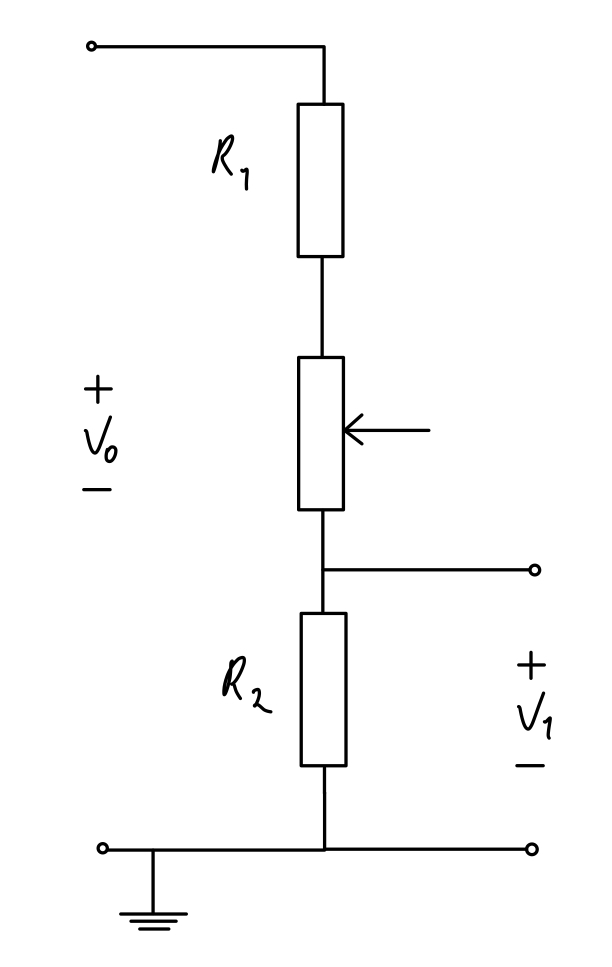
\includegraphics[height=0.4\textwidth]{D1/Images/kretsskjema.jpg} 
  \caption{Inngang $v_0$ med motstander $R_1$, $R_2$, potensiometer og utgang $v_1$.}
  \label{fig:kretsskjema}
\end{figure}
Ved å gå ut ifra at potensiometer har en maksimum og minimum kan vi regne ut motstandsverdiene for å oppnå ønsket demping ved å løse likningssettet for spenningsdeling i (\ref{eq:pot0}) og (\ref{eq:pot1}), med motstandene $R_1$ og $R_2$ som ukjente. I likning (\ref{eq:pot0}) er potensiometeret ($R_P$) justert ned til laveste mulig motstand, mens i likning (\ref{eq:pot1}) er det justert opp til høyeste mulig motstand. 
\begingroup
\Large
\begin{equation}
    \frac{R_1}{R_1+R_2} = A_{min} 
    \label{eq:pot0}
\end{equation}
\begin{equation}
    \frac{R_1}{R_1+R_2+R_P} = A_{max} 
    \label{eq:pot1}
\end{equation}
\endgroup

Likningsettet kan løses til formlene vist i (\ref{eq:los1}) og (\ref{eq:los2}) for å finne $R_1$ og $R_2$.

\begingroup
\Large
\begin{equation}
    R_1 = \frac{A_{min}A_{max}R_P}{A_{min}-A_{max}}
    \label{eq:los1}
\end{equation}
\begin{equation}
    R_2 = -\frac{(A_{min}-1)A_{max}R_P}{A_{min}-A_{max}}
    \label{eq:los2}
\end{equation}
\endgroup

% \begin{equation}
%     -20 dB = 20 \log  A_{min} \xrightarrow[]{}  A_{min} = 0.1
% \end{equation}
% \begin{equation}
%     -5 dB = 20 \log  A_{max} \xrightarrow[]{}  A_{max} = 0.562
% \end{equation}
\section{Realisering og test}
\label{sec:realisering}
Nivåregulatoren realiseres med $A_{min} = -5 \text{dB}$ til $A_{max} = -20 \text{dB}$ som kravspesifikasjoner og et potensiometer med variabel motstand mellom $0$ og $10.27\text{k}\Omega$. Desibelverdiene må konverteres til spenningsforhold innenfor gitt avvik på 0.1 dB. 
\begingroup
\Large
\begin{equation}
    \label{eq:spenningsforhold}
    A[\text{dB}] = 20\log{A}
\end{equation}
\endgroup 

Ved å bruke likningen (\ref{eq:spenningsforhold}) kan $A_{min}$ og $A_{max}$ regnes ut til
\begingroup
\Large
\begin{align*}
    0.09 < A_{min} < 0.10
\end{align*}
\begin{align*}
    0.57 < A_{max} < 0.56
\end{align*}
\endgroup
Med disse verdiene gir formelene (\ref{eq:los1}) og (\ref{eq:los2}) motstands verdiene
\begingroup
\Large
\begin{align*}
    R_1 \approx 1249.2 \Omega
\end{align*}
\begin{align*}
    R_2 \approx 982.6 \Omega
\end{align*}
\endgroup

Da det er vanskelig å finne nøyaktig disse motstandsverdiene kan det kobles opp med flere motstander av forskjellige verdier i parallell og serie. Standard motstander har ofte en viss feilmargin, dermed er det nødvendig å måle hver enkel motstand med et ohmmeter.

\begin{table}[h]
  \centering
  \caption{Oppgitte og målte verdier med et multimeter med sum nederst.}
  \begin{tabular}{|c|c|c|c|}
    \hline\hline
    Teoretisk verdi $R_1$ & Målt verdi $R_1$ & Teoretisk verdi $R_2$ & Målt verdi $R_2$ ($\Omega$) \\
    \hline\hline
    $1000$ & $982$ & $1000$ & $972$\\
    & & $100$ & $98$\\
    & & $100$ & $98$\\
    & & $100||100$ & $49$\\
    & & $33$ & $32$ \\
    \hline\hline
    $1000$ & $982$ & $1283$ & $1249$\\
    \hline\hline
  \end{tabular}
  \label{tabel:seriemotstander}
\end{table}

Et eksempel på hvordan man kan oppnå motstandverdiene $R_1$ og $R_2$ er realisert i figur (\ref{fig:oppkobling.jpg}), med tabell (\ref{tabel:seriemotstander}) som viser hvilke motstander som blir brukt. Spenningskilden avga i denne realiseringen $V_1$ =  $5.21$V som ga målingene $V_2$ = 0.52V når potensiometeret var skrudd opp til $10.27$k$\Omega$ ($A_{max}$), og 2.92V når det det var skrudd ned til 0$\Omega$ ($A_{min}$).
Disse målingene tilsvarer en amplifikasjon på $A_{max}$ =  $-20.02$dB og $A_{min}$ = $-5.03$dB, som er innenfor systemkravene gitt med avvik mindre enn 0.1dB.  
Mulig årsak til avvik kan være unøyaktig måling med multimeteret, ustabil spenningskilde eller defekte komponenter. 

\begin{figure}
  \centering
  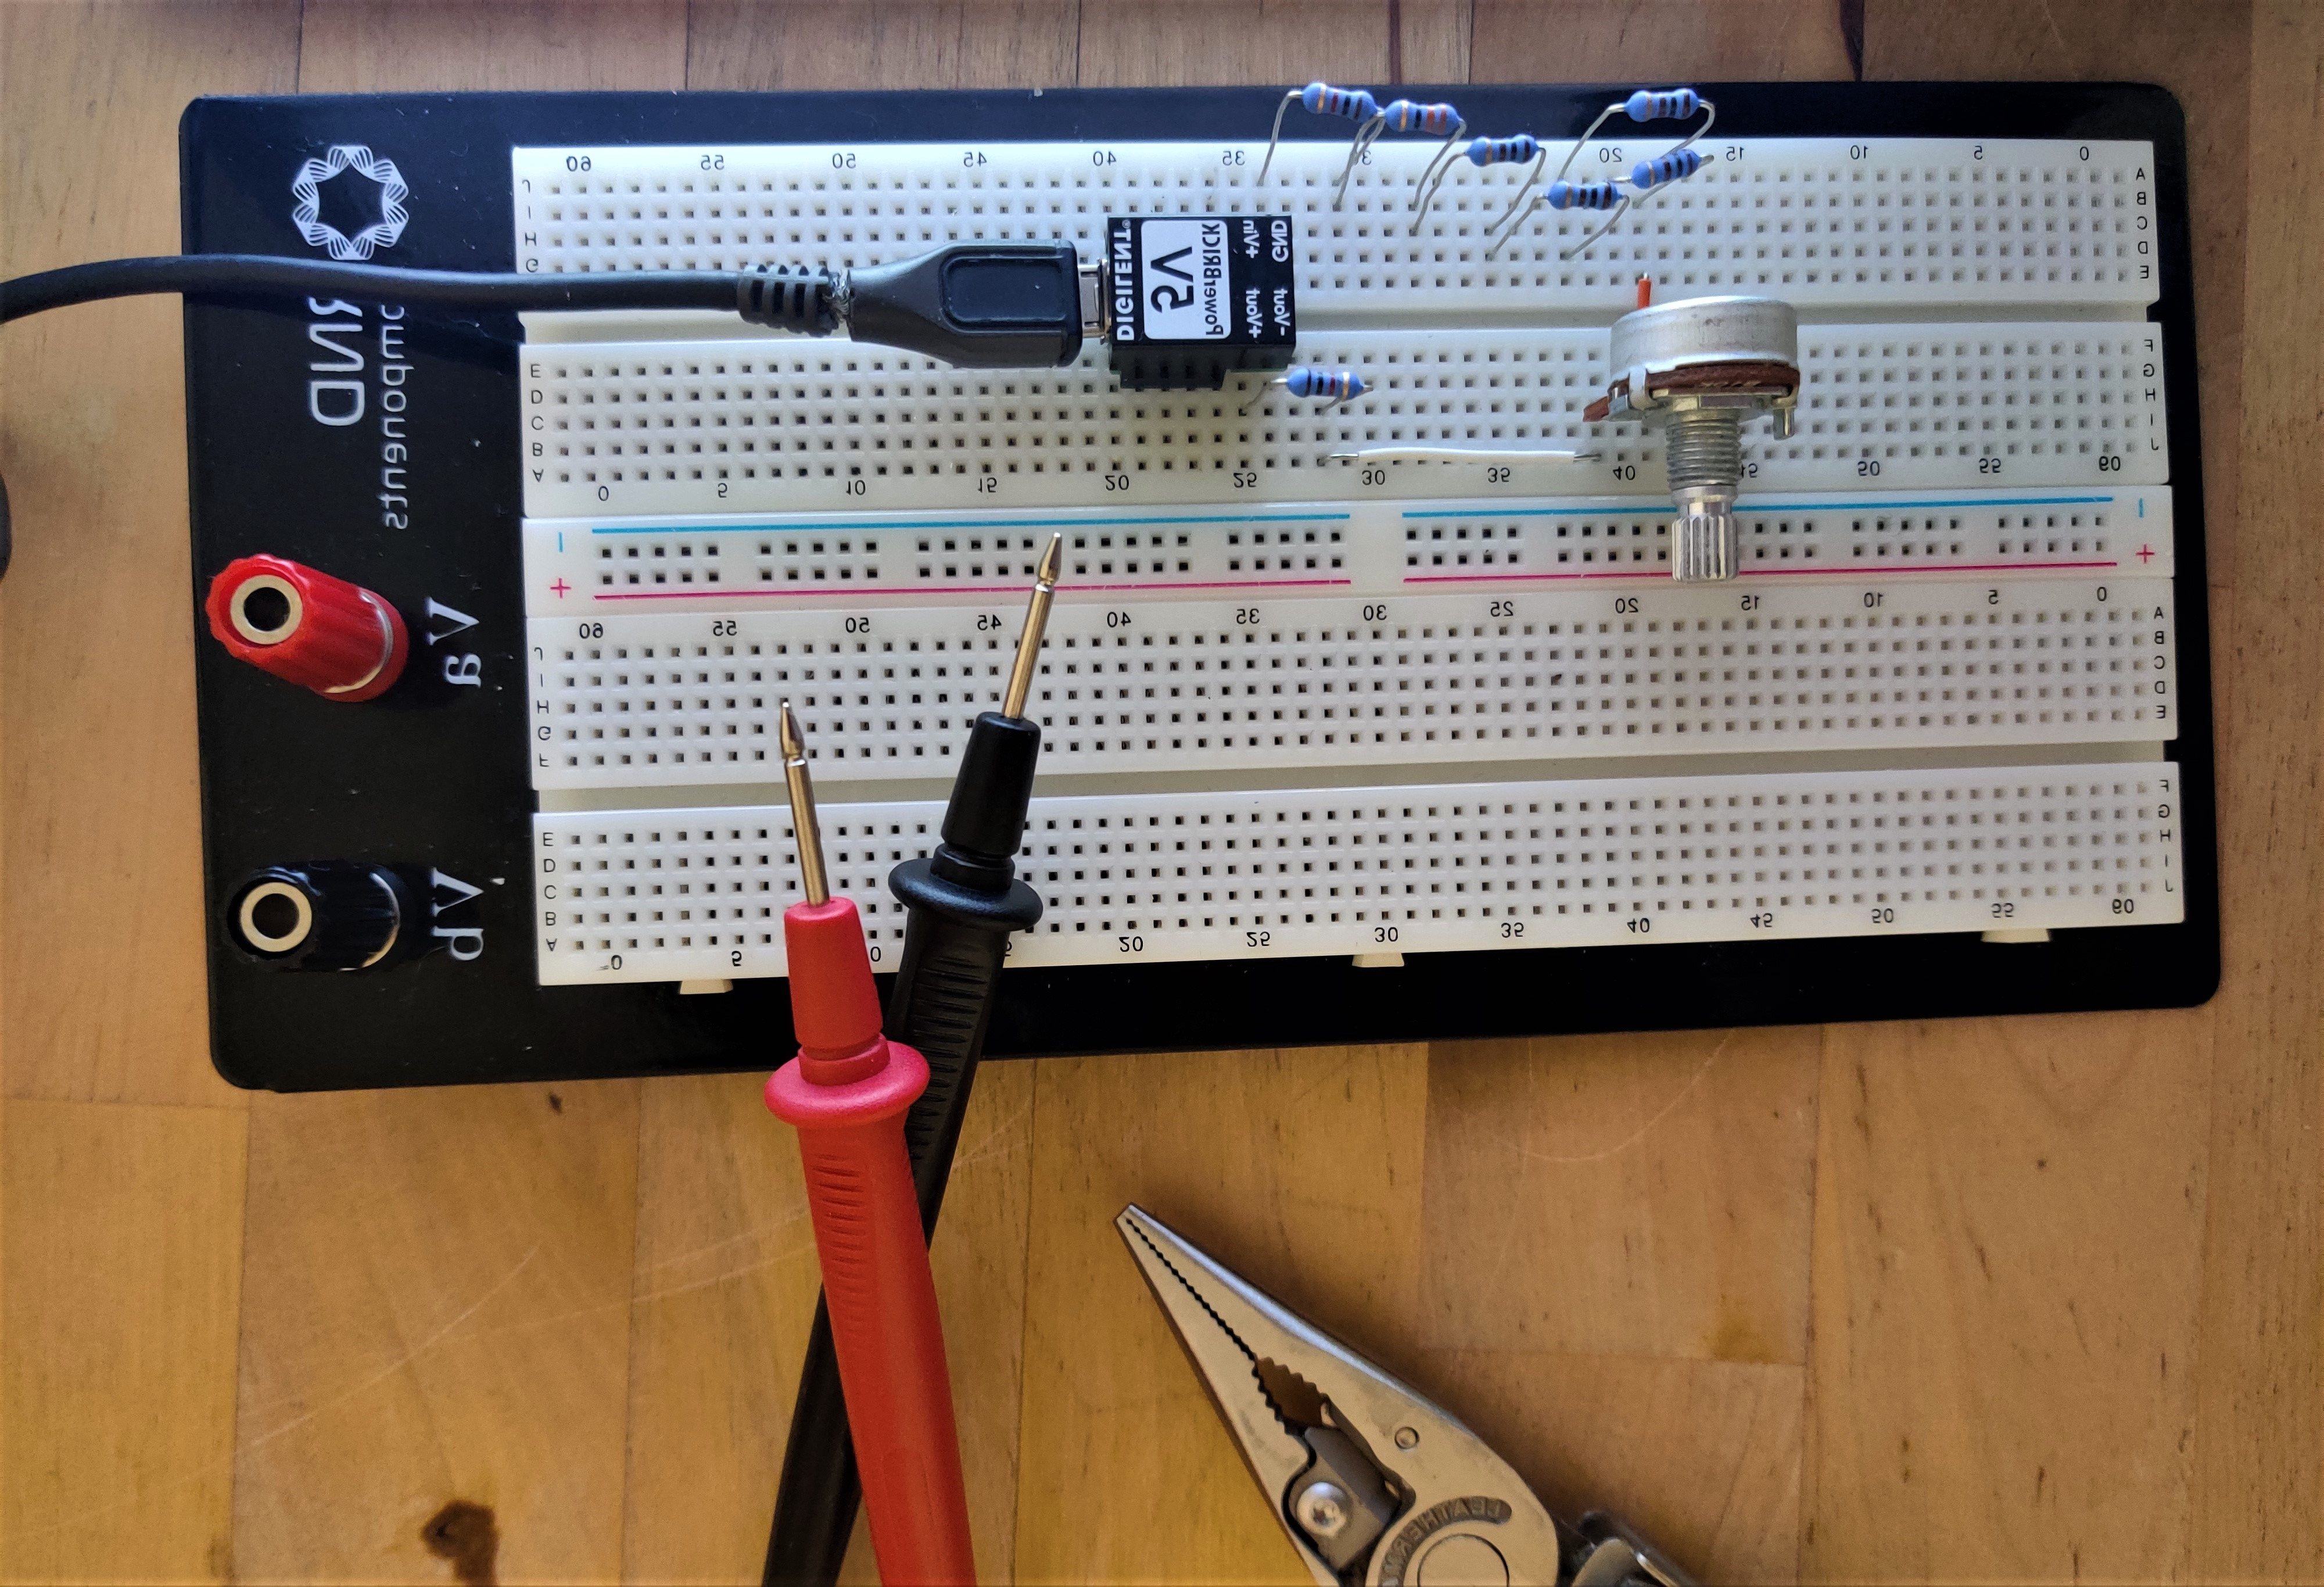
\includegraphics[scale=0.1]{D1/Images/oppkobling.jpg}
  \caption{Nivåregulator som tar inn et signal $v_0$ og gir ut signalet $v_1$.}
  \label{fig:oppkobling.jpg}
\end{figure}

\section{Konklusjon}
\label{sec:konklusjon}
Systemet som ble beskrevet og implementert i dette notatet var en nivåregulator med hensikt om å dempe inngangsignalet til bestemte verdier spesifisert i problembeskrivelsen. Etter testing og realisering ga nivåregulatoren ut en signal med et avvik på mindre enn 0.04dB fra systemkravene.

Oppgitte verdier på motstander er sjeldent pålitelige, dermed må hver enkelt motstand måles for å oppnå en nøyaktig verdi. Dette gjelder også for potensiometeret og spenningskilden da disse også kan avvike fra oppgitt verdi.

\section{Takk}
Takk til Orbit NTNU for å gi meg muligheten til bruk av lokalet og alt nødvendig utstyr, samt hjelp av flere medlemmer. 

Takker også mine medstudenter Mahdan Gazimagamev og Nikolai Andresen for hjelp til feilsøking og produktiv diskusjon rundt prosjektet. 
%Bibliografi: Legg til flere elementer ved å legge til flere \bibitem:--------
\phantomsection
\addcontentsline{toc}{section}{Referanser}
\begin{thebibliography}{99}

\bibitem{notat}
  Lars Lundheim,
  \emph{Variabel nivåregulator},
  Teknisk notat,
  Elsys-2017-LL-1,
  NTNU 2017.

\end{thebibliography}




\end{document}